\documentclass[letterpaper]{physor2024}

%%% Packages Required by Class (already included) TODO figure out....
% \usepackage{fancyhdr}
% \usepackage{lastpage}
% \usepackage{titling}
% \usepackage{titlesec}
% \usepackage{ragged2e}
% \usepackage{enumitem}
% \usepackage{amsmathv}
% \usepackage{graphicx}
% \usepackage{geometry}
% \usepackage{newtxtext}
% \usepackage{newtxmath}
% \usepackage{hyperrefv}
% \usepackage{cleveref}
% \usepackage{caption}
% \usepackage{authblk}
% \usepackage{apptools}
% \usepackage{appendix}
% \usepackage{ifpdf}
% \usepackage{epstopdf}

%%% Some other useful packages
% \usepackage{tikz}
% \usepackage{color}
% \usepackage{subcaption}
% \usepackage{algcompatible}
% \usepackage{bm}
% \usepackage{array}

% \usepackage{nomencl} % If needed
% \makenomenclature


\title{Depletion Analysis of the Virtual Test Bed's Gas-Cooled Microreactor Using OpenMC}

%%% Authors (use arabic numbers: 1, 2, 3, etc. for affiliationNumber)
%%% \addAuthor{GivenName MiddleInitial. FamilyName}{affiliationNumber}
\addAuthor[ligross@wissc.edu]{Lewis I. Gross}{1}
\addAuthor{Paul P.~H. Wilson}{1}

%%% Affiliations (from authblk)
%%% \addAffiliation{affiliationNumber}{Name of Institute, City, State/Country}
\addAffiliation{1}{University of Wisconsin - Madison, Madison, Wisconsin}

%%% Write text for abstract
%%% Most text modifying commands will work in abstract
\Abstract{%
A required 200-250 words abstract should be given here. Use the \texttt{$\backslash$Abstract} command prior to the \texttt{$\backslash$begin\{document\}} command.
The abstract highlights the main accomplishments, what is new, and how it relates to the state-of-the-art.
}

%%% List up to 5 keywords separated by a comma
\keywords{TRISO, depletion, microreactor, gas-cooled, OpenMC}

%%% Provide a short title for the header on odd pages
\shortTitle{PHYSOR 2024 Full Summary Template}

%%% Provide a short author listing for the header on even pages
\authorHead{Hi}

%%% If LaTeX reports the line number of an error at \begin{document} it
%%%   is most likely due to an error in one of the commands above
\begin{document}

\section{Introduction}\label{sec:1}
Introduce the topic of the work in this section.
Use style ``Heading 1'' for section titles. Use 8.5" ×11" paper size, with 1" margins on all sides.

Use style ``Normal'' for the main text of the paper.
Use the IEEE reference style for journal paper \cite{journal}, proceeding paper \cite{conf_paper}, book \cite{book}, and website \cite{website}.
References to websites are discouraged. It is the author’s responsibility to check links in the PDF file of the paper.
All references should be cited in the text in numerical order, in order of appearance as \cite{book,website,proc_paper}. An automatic reference manager, such as Zotero, is recommended.

The full paper should be laid out and formatted according to this template.
Because the paper will be included as a .pdf file for the proceedings, the author will get the best results from Word or WordPerfect by using the Acrobat Distiller or Acrobat PDFWriter as the default printer.
When creating the PDF version, check the ``Embed All Fonts'' option.
Note that it is the author's responsibility to review the final PDF version of the paper to ensure proper translation into PDF.
Final PDF file size should be no more than 4 MB.
Recommended paper length is 8-10 pages.
The limit for full-paper submissions is 10 pages, including references, tables, and figures.
If an exception is made and a paper over 10 pages is accepted, page charges are \$100/page for p. 11 and above.

Do not include bookmarks or hyperlinks to references, figures, and tables in the text of your paper in your final PDF document.
Do not include highlighting, page numbers, headers, or footers.
Disclaimers or information about the author’s employer should not be set as a footer or header.
Instead, set as an end-of-paper note (preferred) or as a footnote that does not interfere with the bottom margin. Do not save your PDF as ``read only.''


\section{Second or Subsequent Major Heading (Font Size 12 Point)} \label{sec:2}

A logical division of the paper into sections, etc., makes it so much easier to understand. All text in this template is ``Normal''.
Make sure to avoid \textbf{\textit{widow/orphan}}  lines.

\subsection{Subsection Title: First Character of Each Non-Trivial Word is Uppercase (12 Point)}
The style for subsection titles and all text in this template is ``Heading 2,'' ``Heading 3,'' etc.
Secondary titles should start flush left and are numbered as illustrated above.

Equations are embedded into tables. Equations should be centered and sequentially numbered to the flush right of the formula using the table provided.
Copy the equation table for additional equations to benefit from automatic numbering.
Use inline equations font with a font size 11 for the text variables and corresponding sizes proportionally for the subscripts and superscripts.
\begin{equation}
    \frac{dM_{c.v.}}{dt} = 0
\end{equation}
where $M_{c.v.}$ and $t$ are the variables in the equation.

\subsubsection{Sub-subsection level and lower: only first character uppercase (12 point)}
Figures and tables should appear as closely as possible to where they are first cited using cross references, e.g., \Cref{fig:sample}, in the text. The figures should be centered. The style for figure captions is ``Caption''. Color is permitted but must be readable if printed in gray scale.
\begin{figure}[h!]
    \centering
    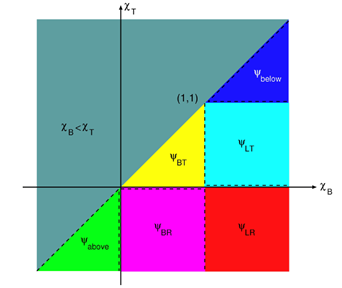
\includegraphics{samplefigure.png}
    \caption{Sample figure.}
    \label{fig:sample}
\end{figure}

When importing figures or any graphical image please verify two things:
\begin{itemize}
    \item Any number, text or symbol is in Times New Roman font and is not smaller than 10 point after reduction to the actual window in the paper.
    \item That it can be translated into PDF.
\end{itemize}

Tables, such as Table I, are numbered in Roman numerals, with the table title in \textbf{boldface} centered above the table with a blank line between the title and actual table. The style for tables is ``Plain Table 2'' found under the ``Table Design'' tab. The style for table captions is ``Table Caption''. The text style for table content is ``Table''.

\begin{table}[h!]
    \centering
    \caption{Sample table.}
    \begin{tabular}{|l|c|c|c|}
        \hline
         \textbf{Mesh}           & \textbf{8 $\times$ 8} & \textbf{16 $\times$ 16} & \textbf{32 $\times$ 32} \\ \hline
         \textbf{Nodal}          & $1.000\times 10^{-1}$ & $2.500\times 10^{-2}$ & $6.250\times 10^{-3}$ \\ \hline
         \textbf{Characteristic} & $1.000\times 10^{-1}$ & $2.500\times 10^{-2}$ & $6.250\times 10^{-3}$ \\ \hline
    \end{tabular}

    \label{tab:sample}
\end{table}

Use SI Units (in parentheses, not square brackets).  Conventional (non-SI) quantities may follow parenthetically if the author desires.  Watch the number of significant digits.

\section{SYSTEM DESCRIPTION}

\section{DEPLETION THEORY}

\section{OPENMC MODEL}

\section{RESULTS}


\section{CONCLUSIONS}
Present summary and conclusions here.

\section*{ACKNOWLEDGEMENTS}
Acknowledge the help of colleagues, and sources of funding, as appropriate.

The first author was supported in part by the US Nuclear Regulatory Commission's Graduate Fellowship Program administered by the University of Wisconsin-Madison.

% \printglossaries

\bibliographystyle{physor2024}
\bibliography{main}

\appendix

\section{}
If necessary, include Appendices numbered in upper case alphabetical order.

To ensure a uniform, professional look at the proceedings, please only modify the format of this template after checking with the publication chair first.


\end{document}